\textbf{Reinforcement learning (RL)} is an area of machine learning that epitomizes the agent-based approach.
RL is unique within its field as it is directly focused on goal-directed learning from agent-environment interaction \cite{rlai}.
At the core of RL lays the reward function (or signal), which perfectly describes goals established by the problem.

In the following chapter, we start by summarizing finite MDPs -- the mathematical underpinning for reinforcement learning, while also familiarizing with the the notation used throughout this paper.

In section \ref{rl:dp} we cover the first solution technique: using dynamic programming in a known, finite MDP to find its optimal solution.
In section \ref{rl:mc}, we generalize this method to solve unknown MDPs -- the complete formulation of a RL problem -- using Monte-Carlo learning.
In section \ref{rl:td}, we visit temporal-difference learning and finally develop our solution using Q-learning in section \ref{rl:q-learning}.

\subsection{Components and Notation}
Introduction into reinforcement learning supposes familiarity with the paradigm's simple-but-effective mathematical framework.
We present the theory behind Markov decision processes (MDPs) and then we shift our attention to explaing the components of a reinforcement learning agent.

\subsubsection{Finite Markov Decision Processes}
Finite Markov decision processes are a formalization of a reinforcement learning problem -- any problem which can be represented as a finite MDP can be solved using a RL technique.

The feedback loop is central to understanding the reinforcement learning dynamic.
This is just a reiteration of the contents in our previous chapter:
an \textbf{agent} acts upon an \textbf{environment}, which reacts according to its set of governing rules.
Each iteration takes place at a discrete time step \(t = 0,1,2,\dots \) (although there are continuous variants of a Markov process, we are not concerned with them).

\begin{figure}[ht]
    \centering
    \caption{Feedback Loop. (Partial reproduction from \cite{rlai})}
    \vspace*{0.2cm}
    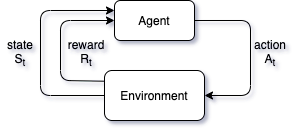
\includegraphics[width=0.5\textwidth]{agent-env-fig}
\end{figure}

\begin{enumerate}
    \item The agent is in state \(s\) and picks action \(a\).
    \item It receives a reward \(r\) for its action. This (immediate) reward signal is problem-defined and quantifies the agent’s goal.
    \item The environment reacts, sending the agent into the next state \(s'\).
\end{enumerate}

A \textbf{Markov decision process (MDP)} is defined as a tuple \(\langle S, A, P, R, \gamma \rangle\), in which:
\begin{enumerate}
    \item \(S\) is the finite set of all states.
    \item \(A\) is the finite set of all possible actions.
    \item \(P\) is the state transition probability function, where \(P_a(s, s')\) denotes the probability of starting in state \(s\) and ending up in state \(s'\) by taking action \(a\).
    \item \(R\) is the reward function, where \(R_a(s, s')\) is a value in \(\mathbb{R}\) and represents the reward received for starting in state \(s\) and ending up in state \(s'\) by taking action \(a\).
    \item \(\gamma\) is the discount factor (used when computing the \textbf{return}), \(\gamma \in [0, 1]\).
\end{enumerate}

The \textbf{state} refers to the internal state of the agent \footnote{Sometimes we may also refer to the state of the environment, but context will clarify. Environment state and agent state only completely match in full observability environments.}.
A state \(S_t\) contains relevant information from the environment at a given time step \(t\).
A key point in Markov processes is that a correctly formulated state captures all the relevant information and removes the need of explicitly memorizing state history.
This is known as the \textbf{Markov property} \cite{silver-lectures}.

A \textbf{policy \(\pi\)} completely characterizes an agent’s behaviour.
``It is a mapping from perceived states of the environment to actions to be taken in those states'' \cite{rlai}.
Policies can be deterministic (i.e. ``if this then that'' rules) or stochastic.
A \textbf{stochastic policy}, denoted \(\pi(a \given s)\), is a probability distribution over actions, given a state.

The \textbf{reward} models the problem-defined goals as a scalar that can be associated with each state transition.
``The reward signal is the primary basis of altering the policy.'' \cite{rlai}.
The assertion that we can completely and correctly model all goals using reward functions is central to the field of RL.
This is called the \textbf{Reward Hypothesis} and is formulated below:
\begin{quotation}
    That all of what we mean by goals and purposes can be well thought of as maximization of the expected value of the cumulative sum of a received scalar signal (called reward). \textit{(from \cite{rlai}, Chapter 3.2)}
\end{quotation}

The \textbf{return} \(G_t\) is the \textbf{cumulative reward} obtained by the agent starting from time step \(t\).
This is what a reinforcement learning system is supposed to maximize.
There are multiple mathematical models used to represent the return.
In equation \ref{eqn:return}, we use an infinite-horizon sum with discounting.

\begin{equation} \label{eqn:return}
    G_t = R_{t+1} + \gamma R_{t+2} + \dots = \sum_{k = 0}^{\infty}{\gamma^{k} R_{t + k + 1}}    
\end{equation}

Discounting is, intuitively, a way to control how much the agent cares about future rewards.
More on this topic can be found in either theoretical reference \cite{rlai, silver-lectures}.

\label{rl:value-func}
The \textbf{state-value function} for policy \(\pi\) is denoted by \(V^{\pi}(s)\) and measures how good each state is, with regard to the long-term potential of that state.
Whereas rewards characterize the immediate value of a state, the value function measures its long-term desirability \cite{rlai}, under the given policy.

\begin{equation} \label{eqn:value}
    V^{\pi}(s) = \mathbb{E}_{\pi}\{ G_t \given S_t = s \}
\end{equation}

Here, \(\mathbb{E}\) represents the expected value (of a random variable) and we denote by \(\mathbb{E}_{\pi}\) the expected value following policy \(\pi\).

An \textbf{action-value function} \(Q^{\pi}(a, s)\) measures the value of a state-action pair and is also known as the Q-value function.
In contrast to the state-value function, the action-value function can be used in unknown MDPs, as it does not depend on its structure.
This is crucial for RL problems as MDPs are typically not known \emph{a priori}.

\begin{equation}
    Q^{\pi}(s, a) = \mathbb{E}_{\pi}\{ G_t \given S_t = s, A_t = a \}
\end{equation}

Value function approximation is the foundation of multiple solution methods in RL. A simple example can be seen in Monte-Carlo methods, where the value of a state \(s\) is approximated by averaging over multiple trajectories starting from \(s\).

A \textbf{model} (of the environment) allows the agent to plan and make predictions of its environment.
Some algorithms focus explicitly on learning a model and use it for \textbf{planning}.
This approach is called \textbf{model-based}.
In a model-based method, an agent can query the model to simulate what would happen with the environment before actually choosing an action.
Approaches without a model are called \textbf{model-free}. Model-free agents are ``explicitly trial-and-error learners'' \cite{rlai}.

\begin{figure}[ht]
    \caption{A way of classifying RL methods based on whether they have a value function, policy or model. (Reproduced from David Silver's lectures. \cite{silver-lectures})}
    \vspace*{0.2cm}
    \centering
    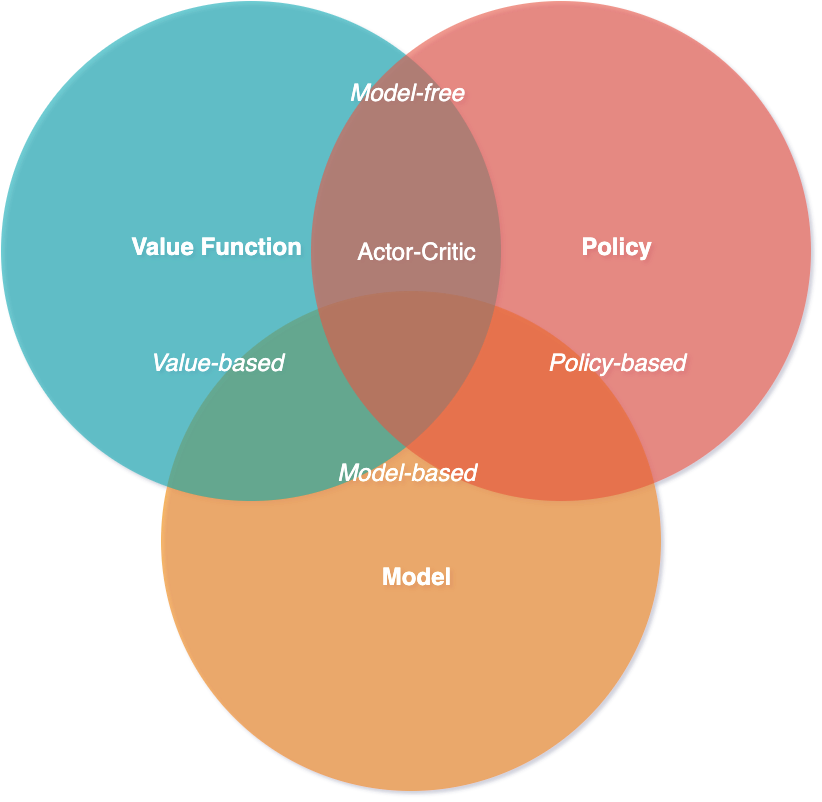
\includegraphics[width=0.5\textwidth]{silver-venn}
\end{figure}

\subsection{Bellman Equations} \label{rl:bellman}
The \textbf{Bellman equations} are a set of relations conceived by Richard Bellman in the 1950s, in the context of solving optimal control using dynamic programming.
The key idea behind the Bellman equations is that they express the value of a state $v(S_{t})$ as \emph{expected sum} of:
\begin{enumerate}
    \item immediate reward of being in that state: $R_{t+1}$.
    \item discounted value of successor state: $\gamma v(S_{t+1})$.
\end{enumerate}

This transformation becomes clear if we use our return-based exprimation of value function $V^{\pi}(s)$ in Equation \ref{eqn:value} and reorganize its terms:

\begin{equation} \label{eqn:bellman-expectation}
\begin{aligned}
    V^{\pi}(s)
        &= \mathbb{E}_{\pi}\{ G_t \given S_t = s \} \\
        &= \mathbb{E}_{\pi}\{ R_{t+1} + \gamma R_{t+2} + \dots \given S_t = s \} \\
        &= \mathbb{E}_{\pi}\{ R_{t+1} + \gamma V^{\pi}(S_{t+1}) \given S_{t} = s \} \\
\end{aligned}
\end{equation}

Equation \ref{eqn:bellman-expectation} states the \textbf{Bellman expectation equation}.
In Figure \ref{fig:expectation-backup}, we model the equation using a backup tree \footnote{Called a backup or update tree, it visualizes the way that state values are updated. This visualization convention is proposed in and used throughout \cite{rlai}.}, where each open circle represents a state, while closed cicles represent state-action pairs.

In state $s$, the agent has a set of available actions according to its policy $\pi$.
After the agent chooses action $a$, the environment responds with reward $r$ and throws the agent into the next state  $s'$ -- one of multiple possible states according to environment dynamics.

Equation \ref{fig:expectation-backup} computes the value of state $s$ by \emph{averaging} over all possible trajectories, \emph{weighing} each by its probability of occuring.

\begin{figure}[ht]
    \centering
    \caption{Bellman expectation backup.} \label{fig:expectation-backup}
    \vspace*{0.2cm}
    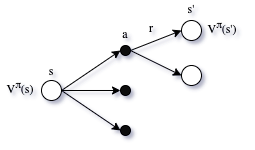
\includegraphics[width=0.4\textwidth]{bellman-expectation-backup}
\end{figure}

In cases in which the MDP is \emph{known}, we can leverage the fact that we know the transition probabilities $P$ to \emph{directly compute} the expectation in \ref{eqn:bellman-expectation}.
\begin{equation}
    \begin{aligned}
        V^{\pi}(s)
            &= \mathbb{E}_{\pi}\{ R_{t+1} + \gamma V^{\pi}(S_{t+1}) \given S_{t} = s \} \\
            &= \sum_{a \in A}{
                \pi(a \given s) ( R(s, a) + \gamma \sum_{s' \in S}{
                    P_a(s, s') V_{\pi}(s')
                })
            }
    \end{aligned}
\end{equation}

There is another important relation, the \textbf{Bellman optimality equation}.
In Chapter \ref{rl:dp} we use it to solve \emph{planning} problems, which require finding the \emph{optimal policy}.
In short, the equation expresses the fact that the value of a state must be the value of the best possible action from that state \cite{rlai}.

\subsection{Dynamic Programming} \label{rl:dp}
\textbf{Dynamic programming (DP)} methods are an important theoretical starting point for reinforcement learning methods. DP problems require full knowledge of an MDP and use general methods to compute optimal solutions.

While being theoretically useful, there are key bottlenecks which prevent DP from achieving practicality:

\begin{enumerate}
    \item DP represents a \textbf{subset} of a reinforcement learning problem, as it requires full knowledge of an MDP and, thus, is not suitable in unknown environments.
    \item DP is \textbf{computationally expensive} as it searches for optimal solutions over the entire state space (suffers from the ``curse of dimensionality'' \cite{rlai}).
    \item DP cannot be applied with \textbf{continuous} spaces, unless problems satisfy additional criteria \cite{rlai}.
\end{enumerate}

There are two key problems that can be solved using DP in a fully known MDP using the Bellman equations.

\textbf{Policy evaluation}, also reffered to as \emph{prediction}, starts with a given policy $\pi$ and is concerned with finding its value function $v_{\pi}$.
In theory, the value of each state can be computed by solving a system of Bellman equations, one for each state.
However, the computation required is impractical for most problems.
A more suitable method is \emph{iterative policy evaluation}, which uses equation \ref{eqn:bellman-expectation} iteratively, starting from an arbitraty value function $v_0$ and eventually converging to $v_{\pi}$.

\textbf{Planning} is, in constrast, concerned with finding the optimal policy $\pi^{\star}$ starting from an arbitraty point in the space.

In order to understand how $\pi^{\star}$ is the \textbf{optimal policy} we need to define an \textbf{ordering} between policies.
Considering $\pi$ and $\pi'$, we say that $\pi' \geq \pi$ if $v_{\pi'}(s) \geq v_{\pi}(s)$ for every $s \in S$.
According this ordering, we say that $\pi^{\star}$ is the optimal policy if its value function is greater than or equal to all other possible policies.

Planning can be done using \emph{policy iteration}.
At every iteration $k$, this method evaluates the given policy $\pi$ to find its value function $v_{\pi}$ (solving the above problem).
Then, it constructs a new policy $\pi'$ which acts \emph{greedily} with regard to $v_{\pi}$.
This is proven to eventually converge to $\pi^*$ as $k \to \infty$ \cite{rlai}.

\begin{figure}[h]
    \caption{An illustration of policy iteration. (From David Silver's lectures. \cite{silver-lectures})}
    \centering
    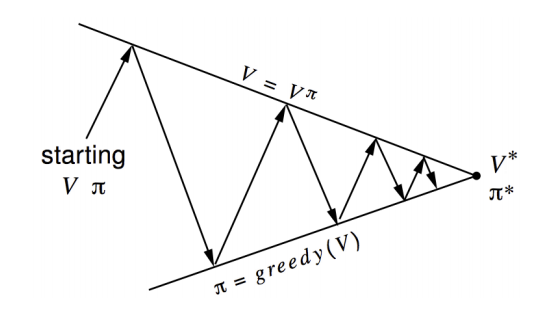
\includegraphics[width=0.4\textwidth]{silver-policy-iteration}
\end{figure}

Using policy iteration can be extremely expensive, as the method adds an additional layer of computation on top of already costly policy evalutation.
The idea of \textbf{value iteration} comes from collapsing the evaluation step with the policy construction step, by applying ``one sweep'' policy iteration -- only updating each value once at every step.

\subsection{Monte-Carlo Learning} \label{rl:mc}

\subsection{Temporal-Difference Learning} \label{rl:td}
TD is a class of solution methods in RL that is part of the model-free subset \cite{rlai}.
An advantage of TD learning can learn from incomplete episodes \cite{long-peak-rl}.

\subsection{Q-Learning} \label{rl:q-learning}
Q-learning \cite{Watkins1992} appeared in 1992 and is considered one of the early breakthroughs of RL \cite{rlai}.
It is a simple algorithm allowing an agent to learn an optimal policy in an unknown environment.